% #### TODO
% ## sistemare graphviz

\documentclass[xcolor=svgnames]{beamer}

% #### graphics and schemes
\usepackage{graphicx}
\graphicspath{{img/}}
\usepackage{tikz}
\usetikzlibrary{shapes,decorations,mindmap,trees}
\usepackage{array}
\usepackage{listings}
\usepackage{ccicons}

% #### theme
\useoutertheme[width=0.16\textwidth]{sidebar}
\useinnertheme{circles}
\usecolortheme{sidebartab}
\usecolortheme{seahorse}
\beamertemplatenavigationsymbolsempty

% #### colors
\usepackage{xcolor}

% #### layouts
\usepackage{multicol}
\usepackage[labelfont=footnotesize,textfont=scriptsize,bf]{caption}
\usepackage{subfig}

% #### math
\usepackage[squaren]{SIunits}

% #### fonts
\usepackage[utf8]{inputenc}
\usepackage[italian]{babel}
\usepackage[T1]{fontenc}
\usepackage{cmbright}
\usepackage{soul} %slanted text
\usepackage{hyperref}
\urlstyle{same}
\hypersetup{pdfauthor={Francesco de Virgilio},pdftitle={OSM e GFOSS: geodati e software liberi in archeologia}}

% #### mainmatter
\title[Geodati e software liberi in archeologia]{OSM e GFOSS: geodati e software liberi\\in archeologia}
\author[Francesco \mbox{de Virgilio}]{Francesco de Virgilio \\ \texttt{\tiny francesco.devirgilio@fradeve.org}}
\institute[GFOSS Day 2011]{GFOSS Day 2011}

%% ##### logo matter ####
\pgfdeclaremask{uniba}{uniba-logo}
\pgfdeclareimage[mask=uniba,width=2cm]{osm-logo}{../img/osm/osm-logo}
\logo{\vbox{\vskip0.1cm\hbox{\pgfuseimage{osm-logo}}}}

\begin{document}

	\begin{frame}
		\begin{center}
			\huge Una settimana con un'azienda archeologica open source
		\end{center}
		\begin{center}
			\includegraphics[width=0.2\textwidth]{../img/archeo/d7}
		\end{center}
	\end{frame}

	% -----------------------------------------------------
	\section{Rilievo}
	% -----------------------------------------------------

		\begin{frame}
			\begin{columns}[c]
				\column{.4\textwidth}
					\begin{center}
						\includegraphics[width=0.8\textwidth]{../img/archeo/1}
					\end{center}
				\column{.6\textwidth}
					\Huge Rilievo
			\end{columns}
		\end{frame}

		% -----------------------------------------------------

		\begin{frame}{Total Open Station\hfill
			\includegraphics[width=0.06\textwidth]{../img/archeo/ita}}{\url{http://tops.iosa.it}\hfill \small{\textbf{Stefano Costa -- Luca Bianconi}}}
			\begin{columns}[c]
				\column{.5\textwidth}
					\begin{center}
						\includegraphics[width=1\textwidth]{../img/archeo/tops}
					\end{center}
				\column{.5\textwidth}
					\begin{itemize}
						\item Leica TCR 1205
						\item Nikon NPL-350
						\item Zeiss Elta R55
					\end{itemize}
			\end{columns}
		\end{frame}

		% -----------------------------------------------------

		\begin{frame}{Neo Freerunner, Debian GNU/Linux}{\url{http://oadigital.net/hardware/openmoko}\hfill \small{\textbf{Oxford Archaeology}}}
			\begin{columns}[c]
				\column{.5\textwidth}
					\begin{center}
						\includegraphics[width=1\textwidth]{../img/archeo/oamoko}
					\end{center}
				\column{.5\textwidth}
					\begin{itemize}
						\item solo software open source
						\item modifiche al sistema operativo
						\item sistemi embedded per l'archeologia
					\end{itemize}
			\end{columns}
		\end{frame}

		% -----------------------------------------------------

		\begin{frame}{GvSIG Mobile su Freerunner}{\url{http://oadigital.net/software/gvsigoade}\hfill \small{\textbf{OA -- GvSIG community}}}
			\begin{columns}[c]
				\column{.5\textwidth}
					\begin{center}
						\includegraphics[width=1\textwidth]{../img/archeo/gvsig_mob}
					\end{center}
				\column{.5\textwidth}
					\begin{itemize}
						\item rilievo emergenze puntuali
						\item collegamento \textit{realtime} tra scavo e ufficio
						\item sync con PostGIS
					\end{itemize}
			\end{columns}
		\end{frame}

	% -----------------------------------------------------
	\section{Documentazione}
	% -----------------------------------------------------

		\begin{frame}
			\begin{columns}[c]
				\column{.4\textwidth}
					\begin{center}
						\includegraphics[width=0.8\textwidth]{../img/archeo/2}
					\end{center}
				\column{.6\textwidth}
					\Huge Documentazione
			\end{columns}
		\end{frame}

		% -----------------------------------------------------

		\begin{frame}{pyArchInit\hfill
			\includegraphics[width=0.06\textwidth]{../img/archeo/ita}}{\url{http://www.adartesnc.com}\hfill \small{\textbf{Luca Mandolesi}}}
			\begin{columns}[c]
				\column{.5\textwidth}
					\begin{center}
						\includegraphics[width=1\textwidth]{../img/archeo/pyarch}
					\end{center}
				\column{.5\textwidth}
					\begin{itemize}
						\item gestione diario di scavo
						\item interrogazione dati georeferenziati
						\item supporto schede US ed esportazione in PDF
						\item generazione matrix
						\item integrazione con QGIS e database
						\item utilizzo intuitivo
					\end{itemize}
			\end{columns}
		\end{frame}

		% -----------------------------------------------------

		\begin{frame}{pyArchInit\hfill
			\includegraphics[width=0.06\textwidth]{../img/archeo/ita}}{\url{http://www.adartesnc.com}\hfill \small{\textbf{Luca Mandolesi}}}
			\includegraphics[width=1\textwidth]{../img/archeo/py}
		\end{frame}

	% -----------------------------------------------------
	\section{Post-processing}
	% -----------------------------------------------------

		\begin{frame}
			\begin{columns}[c]
				\column{.4\textwidth}
					\begin{center}
						\includegraphics[width=0.8\textwidth]{../img/archeo/3}
					\end{center}
				\column{.6\textwidth}
					\Huge Post\\processing
			\end{columns}
		\end{frame}

		% -----------------------------------------------------

		\begin{frame}{QGIS + plugins\hfill
			\includegraphics[width=0.06\textwidth]{../img/archeo/ita}}{\url{wiki.uibk.ac.at/confluence/display/excavationtutor}\hfill\small{\textbf{QGIS community}}}
			\begin{columns}[c]
				\column{.5\textwidth}
					\begin{center}
						\includegraphics[width=1.1\textwidth]{../img/archeo/qgis}
					\end{center}
				\column{.5\textwidth}
					\begin{itemize}
						\item suite GIS open source completa
						\item set di plugins sempre aggiornato
						\item conforme agli standard aperti
						\item utilizzo intuitivo
						\item ottima documentazione
						\item numerosi casi di utilizzo in archeologia
					\end{itemize}
			\end{columns}
		\end{frame}

		% -----------------------------------------------------

		\begin{frame}{GRASS GIS}{\url{http://grass.osgeo.org/wiki/Archaeology}\hfill\small{\textbf{GRASS community}}}
			\begin{columns}[c]
				\column{.5\textwidth}
					\begin{center}
						\includegraphics[width=1.1\textwidth]{../img/archeo/grass.pdf}
					\end{center}
				\column{.5\textwidth}
					\begin{itemize}
						\item suite GIS open source completa
						\item radiazione solare: potenziali insediamenti
						\item analisi LIDAR
						\item visualizzazione ed estrusione edifici 3D
						\item interpolazione 2D e 3D
						\item analisi viewshed
					\end{itemize}
			\end{columns}
		\end{frame}

		% -----------------------------------------------------

		\begin{frame}{\textit{GRASS GIS in archeologia\hfill
			\includegraphics[width=0.06\textwidth]{../img/archeo/ita}}}{\url{http://openoia.org/blog/portfolio/grass-book}\hfill\small{\textbf{O.I.A.}}}
			\begin{columns}[c]
				\column{.5\textwidth}
						\includegraphics[trim=60pt 0pt 0pt 0pt,clip=true,width=1\textwidth]{../img/archeo/grass-arch.pdf}
				\column{.5\textwidth}
					libro collaborativo sull'utilizzo di GRASS in archeologia		
					\begin{itemize}
						\item licenza libera (GFDL)
						\item sorgente disponibile
						\item lingua italiana
						\item versione stampabile (\LaTeX) e web
					\end{itemize}
			\end{columns}
		\end{frame}

	% -----------------------------------------------------
	\section{Gestione}
	% -----------------------------------------------------

		\begin{frame}
			\begin{columns}[c]
				\column{.4\textwidth}
					\begin{center}
						\includegraphics[width=0.8\textwidth]{../img/archeo/4}
					\end{center}
				\column{.6\textwidth}
					\Huge Gestione
			\end{columns}
		\end{frame}

		% -----------------------------------------------------

		\begin{frame}{ARK}{\url{http://ark.lparchaeology.com}\hfill\small{\textbf{L.--P. Archaeology}}}
			\begin{center}
				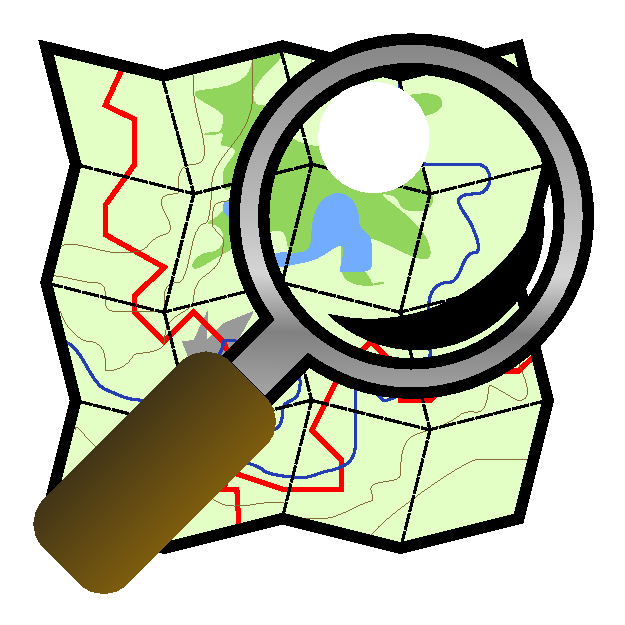
\includegraphics[width=0.3\textwidth]{../img/archeo/logo}
			\end{center}

			ARK (\emph{Archaeological Recording Kit}) è un sistema open source, aderente agli standard e basato sul web, per la creazione, archiviazione, manipolazione e pubblicazione di dati e contenuti multimediali archeologici.\\

			In altre parole, è un sistema che può essere utilizzato per pubblicare dati archeologici sul web, per la collaborazione e la condivisione sul web.
		\end{frame}

		% -----------------------------------------------------

		\begin{frame}{ARK}
			\framesubtitle{Caratteristiche\hfill\small{\textbf{L.--P. Archaeology}}}
			\begin{description}
				\item[web-based] set di strumenti per inserimento, modifica, condivisione di documentazione archeologica
				\item[flessibile]struttura dati modificabile in base alle esigenze (compatibile con qualsiasi scheda US/SCR)
				\item[open source] LAMP (Linux/Apache/MySQL/PHP)
			\end{description}
			\vfill
			\begin{center}
				\textbf{\url{http://www.fastionline.org}}
			\end{center}
		\end{frame}

		% -----------------------------------------------------

		\begin{frame}{ARK}
		\framesubtitle{Screenshot\hfill\small{\textbf{L.--P. Archaeology}}}
			\begin{figure}
				\centering
				\caption[\emph{Data entry} in Ark.]{\emph{Data entry} in Ark.}
				\includegraphics[width=0.8\textwidth]{../img/archeo/ark_data_entry}
				\label{fig:data_entry}
			\end{figure}
		\end{frame}

		% -----------------------------------------------------

		\begin{frame}{ARK}
		\framesubtitle{Screenshot\hfill\small{\textbf{L.--P. Archaeology}}}
			\begin{figure}
				\centering
				\caption[Vista dei \emph{record} in Ark.]{Vista dei \emph{record} in Ark.}
				\includegraphics[width=0.7\textwidth]{../img/archeo/ark_record_view}
				\label{fig:data_entry}
			\end{figure}
		\end{frame}

		% -----------------------------------------------------

		\begin{frame}{ARK}
		\framesubtitle{Screenshot\hfill\small{\textbf{L.--P. Archaeology}}}
			\begin{figure}
				\centering
				\caption[Elenco US/SCR in Ark.]{Elenco US/SCR in Ark.}
				\includegraphics[width=0.7\textwidth]{../img/archeo/ark_register}
				\label{fig:data_entry}
			\end{figure}
		\end{frame}

		% -----------------------------------------------------

		\begin{frame}{Graphviz\hfill
			\includegraphics[width=0.06\textwidth]{../img/archeo/ita}}{\url{http://www.iosa.it/content/harris-matrix-graphviz}}
			\begin{columns}[c]
				\column{.5\textwidth}
					\begin{center}
						\includegraphics[width=0.55\textwidth]{../img/archeo/matrix}
					\end{center}
				\column{.5\textwidth}
					\begin{itemize}
						\item notevole automazione
						\item scripting
						\item editabile con qualsiasi software
						\item linguaggio descrittivo
					\end{itemize}
			\end{columns}
		\end{frame}

	% -----------------------------------------------------
	\section{Analisi}
	% -----------------------------------------------------

		\begin{frame}
			\begin{columns}[c]
				\column{.4\textwidth}
					\begin{center}
						\includegraphics[width=0.8\textwidth]{../img/archeo/5}
					\end{center}
				\column{.6\textwidth}
					\Huge Analisi
			\end{columns}
		\end{frame}

		% -----------------------------------------------------

		\begin{frame}{R\hfill
			\includegraphics[width=0.06\textwidth]{../img/archeo/ita}}{\url{http://wiki.iosa.it/sum_of_individual_weighted_means}}
			\begin{columns}[c]
				\column{.5\textwidth}
					\begin{center}
						\includegraphics[width=1\textwidth]{../img/archeo/parkercomparison}
					\end{center}
				\column{.5\textwidth}
					\begin{itemize}
						\item scriptabile
						\item permette lo scambio dati tra GRASS e PostgreSQL
						\item esporta in formati standard (svg)
					\end{itemize}
			\end{columns}
		\end{frame}

	% -----------------------------------------------------
	\section{Esportazione}
	% -----------------------------------------------------

		\begin{frame}
			\begin{columns}[c]
				\column{.4\textwidth}
					\begin{center}
						\includegraphics[width=0.8\textwidth]{../img/archeo/6}
					\end{center}
				\column{.6\textwidth}
					\Huge Esportazione
			\end{columns}
		\end{frame}

		% -----------------------------------------------------

		\begin{frame}{\LaTeX}{\url{http://www.latex-project.org/}}
			\begin{columns}[c]
				\column{.5\textwidth}
					\begin{center}
						\includegraphics[width=1\textwidth]{../img/archeo/laurana}
					\end{center}
				\column{.5\textwidth}
					\begin{itemize}
						\item linguaggio di markup versatile
						\item scriptabile
						\item eccellenti risultati tipografici
						\item integrazione di mesh 3D (\href{http://ctan.org/tex-archive/macros/latex/contrib/movie15/}{pacchetto \texttt{movie15}})
						\item realizzazione di schede US
					\end{itemize}
					vedi anche \url{http://www.reportlab.com} (Python)
			\end{columns}
		\end{frame}

		% -----------------------------------------------------

		\begin{frame}{Mapnik}{\url{http://mapnik.org}}
			\begin{center}
				\includegraphics[width=0.8\textwidth]{../img/archeo/cerveteri_mapnik}
				\begin{itemize}
					\item rendering cartografico di qualità
					\item altamente customizzabile
					\item python bindings
					\item desktop / webgis
				\end{itemize}
			\end{center}
		\end{frame}

	% -----------------------------------------------------
	\section{Didattica}
	% -----------------------------------------------------

		\begin{frame}
			\begin{columns}[c]
				\column{.4\textwidth}
					\begin{center}
						\includegraphics[width=0.8\textwidth]{../img/archeo/7}
					\end{center}
				\column{.6\textwidth}
					\Huge Didattica e comunicazione
			\end{columns}
		\end{frame}

		% -----------------------------------------------------

		\begin{frame}{Textpattern}{\url{http://textpattern.com/}}
			\begin{center}
				\includegraphics[width=0.8\textwidth]{../img/archeo/thames}
			\end{center}
			Discover Thames project\hfill\url{www.thamesdiscovery.org}
		\end{frame}

		% -----------------------------------------------------

		\begin{frame}{GeoServer + OpenLayers + OpenStreetMap\hfill
			\includegraphics[width=0.06\textwidth]{../img/archeo/ita}}{\url{http://geoserver.org} + \url{www.openlayers.org}}
			\begin{center}
				\includegraphics[width=0.9\textwidth]{../img/archeo/fotouring}
			\end{center}
			Lazio Fotouring\hfill\url{www.futouring.com}
		\end{frame}

	% -----------------------------------------------------
	\section{Perchè?}
	% -----------------------------------------------------

		\begin{frame}
			\begin{columns}[c]
				\column{.4\textwidth}
					\begin{center}
						\includegraphics[width=0.8\textwidth]{../img/archeo/question}
					\end{center}
				\column{.6\textwidth}
					\Huge Perché perderci la testa?
			\end{columns}
		\end{frame}

		% -----------------------------------------------------

		\begin{frame}{Software libero: indipendenza dell'utente}
			\begin{columns}[c]
				\column{.5\textwidth}
					\begin{center}
						\includegraphics[width=1\textwidth]{../img/archeo/hello1}
					\end{center}
				\column{.5\textwidth}
					\begin{center}
						\includegraphics[width=1\textwidth]{../img/archeo/hello2}
					\end{center}
			\end{columns}
			\vfill
			\begin{center}
				Possibilità di adattamento / estensione\\tramite moduli / plugin
			\end{center}
			\end{frame}

		% -----------------------------------------------------

		\begin{frame}{Etica}
			\begin{columns}[c]
				\column{.5\textwidth}
					Libertà di:
					\begin{itemize}
						\item espressione
						\item confronto
						\item dialogo
					\end{itemize}
				\column{.5\textwidth}
					Didattica:
					\begin{itemize}
						\item libertà di distribuzione del software
						\item libertà di distribuire versioni modificate
						\item docenti e studenti sullo stesso piano
					\end{itemize}
			\end{columns}
		\end{frame}

		% -----------------------------------------------------

		\begin{frame}{Vantaggi economici}
			\begin{center}
				\includegraphics[width=0.3\textwidth]{../img/archeo/gratis}
			\end{center}
		\end{frame}

		% -----------------------------------------------------

		\begin{frame}{Mercato del lavoro}
			\begin{center}
				\includegraphics[width=0.52\textwidth]{../img/archeo/linked_grass}
				\hfill
				\includegraphics[width=0.48\textwidth]{../img/archeo/linked_oracle}\\
				\includegraphics[width=0.55\textwidth]{../img/archeo/linked_gmaps}\\
				Fonte: LinkedIn Skills, Nov 2011
			\end{center}
		\end{frame}

	% -----------------------------------------------------
	% -----------------------------------------------------

	\begin{frame}{Grazie!}\label{sli:grazie}
		\begin{center}
			\Huge{Thanks for your time}
			\vfill
			\begin{tikzpicture}[cap=round]
			% Colors
			\colorlet{anglecolor}{green!50!black}
			\colorlet{bordercolor}{black}

			\def\alpha{5} % degree
			\def\layer{5}

			\begin{scope}[scale=1.5]
			\pgfmathsetmacro\sinTriDiff{sin(60-\alpha)}
			\pgfmathsetmacro\cosTriDiff{1-cos(60-\alpha)}
			\pgfmathsetmacro\radiusC{sqrt(\cosTriDiff*\cosTriDiff + \sinTriDiff*\sinTriDiff)}
			\pgfmathsetmacro\startAng{\alpha + atan(\sinTriDiff/\cosTriDiff)}

			\pgfmathsetmacro\al{\alpha*\layer}

			\foreach \x in {0,\alpha,...,\al}
			{
			  \pgfmathsetmacro\ang{\x + \startAng}
			  \pgfmathsetmacro\xRs{\radiusC*cos(\ang)}
			  \pgfmathsetmacro\yRs{\radiusC*sin(\ang)}

			  \pgfmathsetmacro\radiusLayer{\xRs + sqrt( 1 - \yRs*\yRs )}

			  \pgfmathsetmacro\angRs{acos(\yRs)}

			  \pgfmathsetmacro\angRss{acos(\radiusC*sin(\ang-\alpha))}


			  \colorlet{anglecolor}{black!\ang!green}

			  \pgfmathsetmacro\step{2*\alpha - 180}
			  \pgfmathsetmacro\stop{180-2*\alpha}
			  \foreach \y in {-180, \step ,..., \stop}
			  {
			    \pgfmathsetmacro\deltaAng{\y-\x}
			    \filldraw[color=anglecolor,draw=bordercolor] 
				(\y-\x:\radiusLayer)    
					arc (-90+\angRs+\deltaAng : \alpha-90+\angRss+\deltaAng :1) 
					arc (\alpha+90-\angRss+\deltaAng : 2*\alpha+90-\angRs+\deltaAng :1)
					arc (\deltaAng+2*\alpha : \deltaAng : \radiusLayer);
			  }



			}
			\pgfmathsetmacro\xRs{\radiusC*cos(\al+\startAng)}
			\pgfmathsetmacro\yRs{\radiusC*sin(\al+\startAng)}
			\pgfmathsetmacro\radiusLayer{\xRs + sqrt( 1 - \yRs*\yRs )}
			\draw[line width=2, color=bordercolor] (0,0) circle (.8*\radiusLayer);
			\pgfmathsetmacro\radiusSmall{.7*\radiusLayer}
			\foreach \x in {-60,0,...,240}
			{
			    \fill[color=anglecolor] (\x:\radiusSmall) arc (-180+\x+60: -180+\x: \radiusSmall)
						     arc (0+\x: -60+\x: \radiusSmall)
						     arc (120+\x: 60+\x: \radiusSmall); 
			}
			\foreach \x in {0, 4, ..., 360}
			{
			  \fill[color=anglecolor] (\x:1) -- (\x+3:1.05) -- (\x+5:1.05) -- (\x+2:1) -- cycle;
			  \fill[color=anglecolor] (\x+5:1.05) -- (\x+7:1.05) -- (\x+4:1.1) -- (\x+2:1.1) -- cycle;
			}
			\draw[line width=1, color=bordercolor] (0,0) circle (1);
			\draw[line width=1, color=bordercolor] (0,0) circle (1.1);
			\end{scope}

			\end{tikzpicture}
			\vfill
			\huge{and keep Geographic FLOSS rockin'}
		\end{center}
	\end{frame}

	% -----------------------------------------------------

	\begin{frame}{Credits and licence}
		\begin{center}
			\Huge{\ccbyncsa}
		\end{center}
		\vfill
		Grazie a:
		\begin{itemize}
			\item Maurizio Napolitano (FBK, Trento -- OKF Italia)
			\item Gfoss.it
			\item Francesco Pelullo (aka \texttt{niubii})
			\item Daniel Steger per ``Mosaic from Pompeii''\footnote{\url{www.texample.net/tikz/examples/mosaic-from-pompeii/}.}, in slide \ref{sli:grazie}
		\end{itemize}
	\end{frame}

\end{document}
